98. $\cfrac{(x-7)\sqrt{x+5}}{x^6-16x^2}\geqslant0\Leftrightarrow
\cfrac{(x-7)\sqrt{x+5}}{x^2(x-2)(x+2)(x^2+4)}\geqslant0.$ Применив метод интервалов, найдём ответ: $x\in\{-5\}\cup(-2;0)\cup(0;2)\cup[7;+\infty).$
\begin{figure}[ht!]
\center{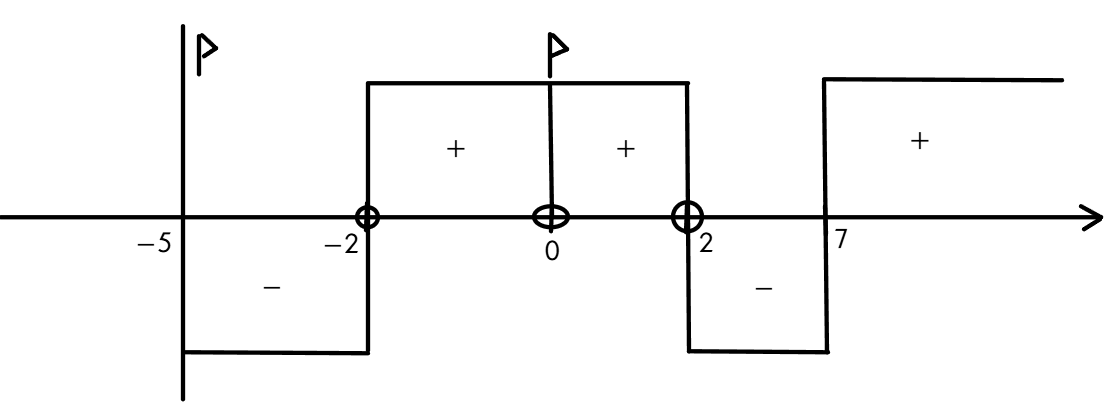
\includegraphics[scale=0.35]{int97.png}}
\end{figure}\\
